\documentclass[a4paper,fleqn,11pt,dvips,titlepage]{article}

\usepackage{amsmath}
\usepackage[utf8]{inputenc}
\usepackage{amsfonts}
\usepackage{amssymb}
\usepackage{geometry}
%\usepackage[english]{babel}
\usepackage{fullpage}
\usepackage{graphicx}
% \usepackage{rotating}
% \usepackage[ps2pdf,colorlinks=false,pdfborder={0 0 0}]{hyperref}
% \usepackage{fancyvrb}
% \usepackage{subfigure}
% \usepackage{url}

\parindent = 0 cm
\parskip = 1.5\medskipamount

\newcommand{\tab}{\hspace{\bigskipamount}}
\newcommand{\ar}[1]{\ensuremath{\hspace{-0.5 ex}\left(#1\right)}}
\newcommand{\ens}[1]{\ensuremath{\left\{#1\right\}}}
\newcommand{\tq}{\ensuremath{\;|\;}}
\newcommand{\R}{\ensuremath{\mathbb{R}}}
\newcommand{\Order}[1]{\ensuremath{\mathcal{O}\ar{#1}}}
\newcommand{\suml}[2]{\ensuremath{\sum\limits_{#1}^{#2}}}
\newcommand{\tuple}[1]{\ensuremath{\left(#1\right)}}

\numberwithin{figure}{section}
\numberwithin{equation}{section}

\newcommand{\ie}{\emph{i.e.}, }


\begin{document}

% \renewcommand{\labelitemi}{\ensuremath{\bullet}}

\newgeometry{margin=0.5cm}
\begin{titlepage}
  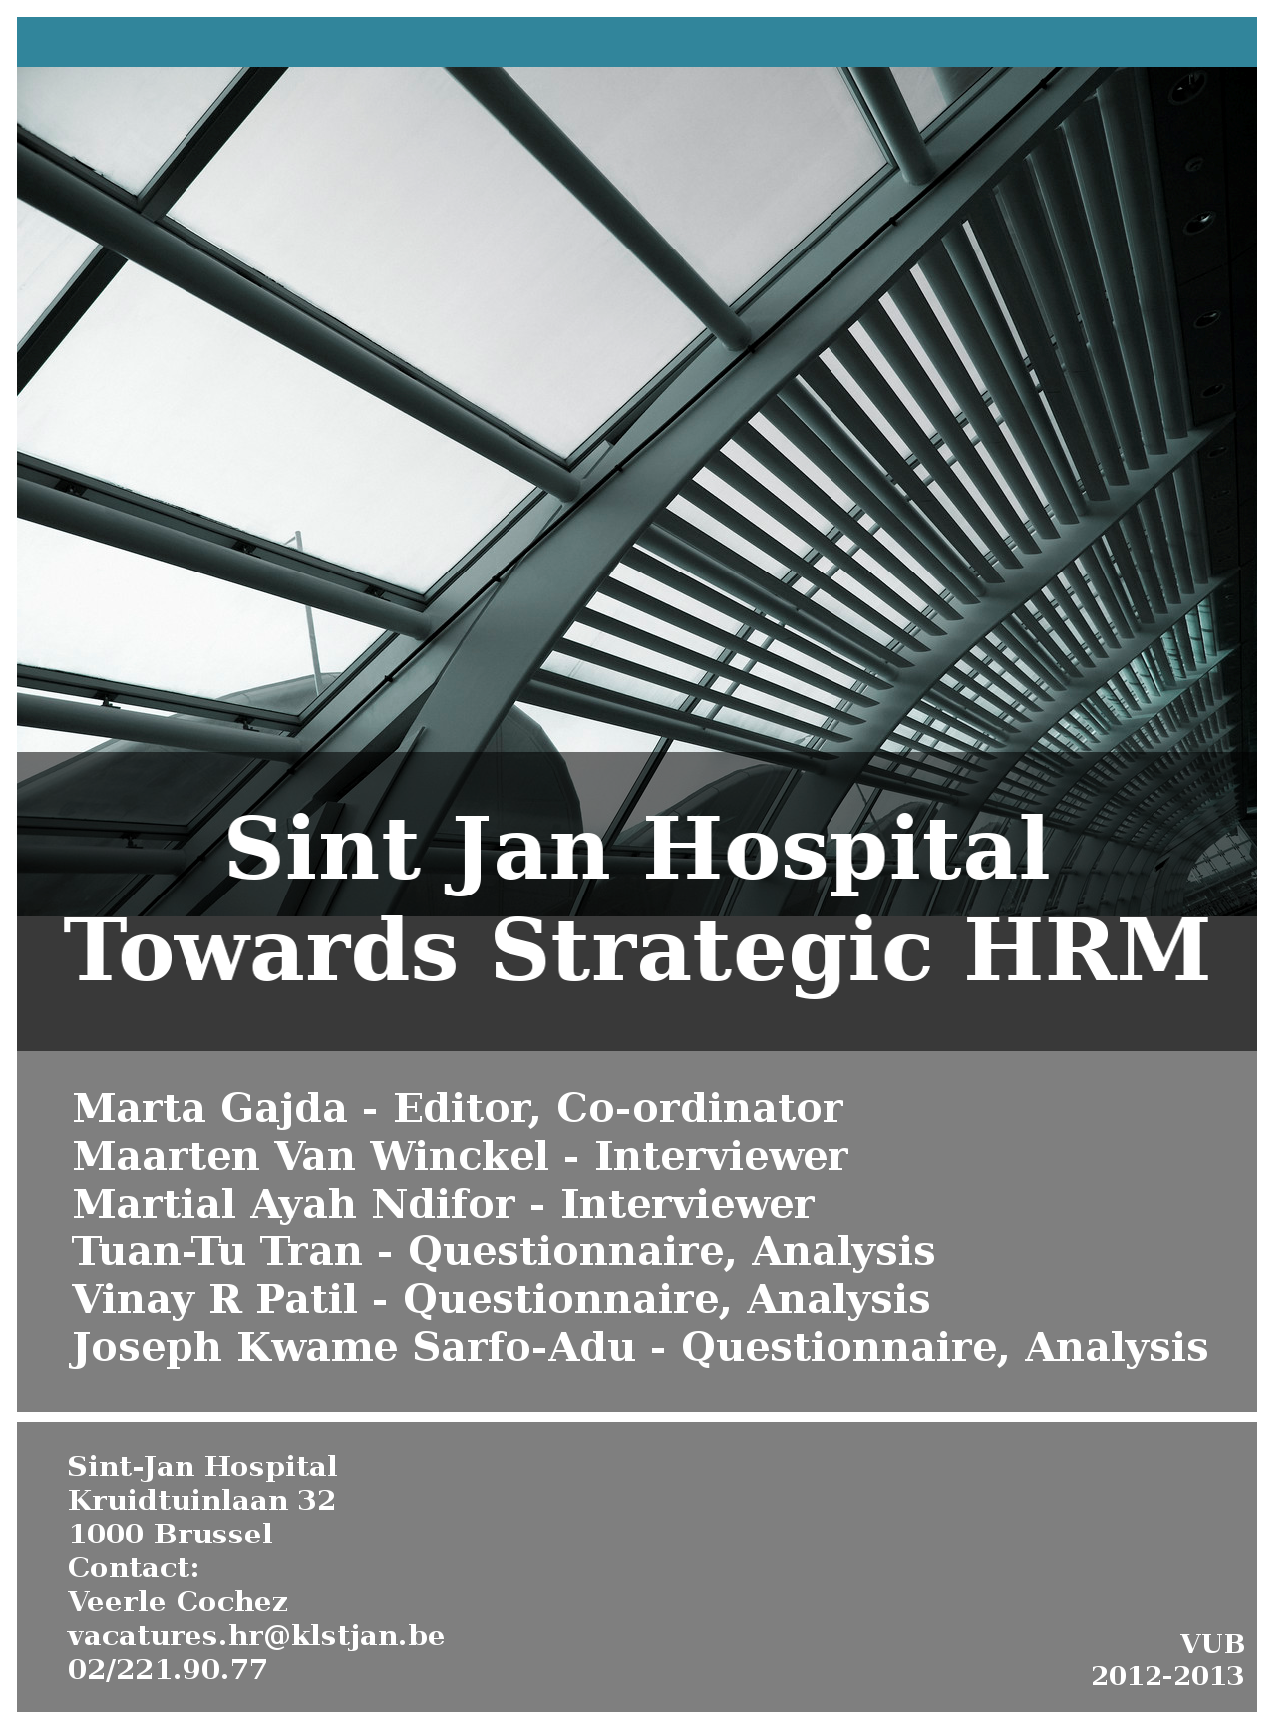
\includegraphics[width=20cm, height=28cm]{cover.eps}
\end{titlepage}
\restoregeometry

\section*{Executive Summary}

\begin{itemize}
  \item Sint Jan hospital is a public health care institution located in Brussels, which employs around 1200 people. Human Resources department is one of six existing in a hospital.
  \item The hospital is not forecasting any major restructuration in the coming years. Recruitments processes are usually adapted to given departments needs. As the organization does not develop any new positions often the same job advertisements are used multiple times.
  \item Candidates are chosen based on the selection criteria. Personality and knowledge of local languages play an important role in the recruitment process. The hiring decision lies within the head of the targeted department. Employees are offered six month probation period, after which a permanent job offer is made.
  \item Sint Jan hospital does not use any social media tools. From the recent research it can be concluded that social networking will be an inevitable of every HR and communication processes. By introducing set of regulations Sint Jan hospital can educate its employees an online etiquette and benefit from the new means of recruitment.
  \item Skills inventory seems essential for institution like the hospital. Many of recruitment processes are conducted internally; skills inventory could facilitate the procedures. It will also help establish plans for any future training. 
  \item Outsourcing can also be beneficial for Sint Jan. It can lower the operating costs, as well as help the human resources department focus on recruitment of high – priority employees. 
\end{itemize}

\newpage

\tableofcontents
\newpage

\section{Introduction}

Since the 1980s human resources management has gained more and more acceptance among scholars and business.
A HRM post is now a vital and often one of the most important part of almost every big company.
Human resources management is mainly responsible for staffing, performance management, workforce development, employee engagement, benefits and workforce investment (Packard). 

However, the term human resources management does not have one applicable definition.
According to Chris Hendry, the HRM does not constitute a unified theory yet.
We can distinguish three major approaches to human resources management.
The first one usually simply states the importance of HRM practice within the company.
The second one, stresses the importance of matching employment practices to an organization’s strategy.
As a result, the employment processes should complement each other, therefore should be integrated through other mechanism, such as personnel planning.
The rewards and promotional systems, training schemes are also part of this kind of approach.
The main goal is to convey a consistent message through HRM practices.
The third approach emphasizes the philosophy of human resources management.
The HRM philosophy consists of high-trust relations, employee commitment and motivation.
The employment practices should be coherent and reflect corporate values (Hendry, 2011).

This paper will focus on the employment strategies applied at the Sint Jan hospital in Brussels.
The paper will shortly describe the organizational structure of the hospital, current human resources management practices and possible ways of improving the HRM department performances.
We will base our analysis on the knowledge gained via an interview with hospital’s employee responsible for recruitment policies. 


\section{Sint Jan Hospital – Organization Structure}

Sint Jan hospital is a public sector hospital located in Brussels.
Hospital has 473 beds and employs around 1200 people.
Organization has 6 functional departments namely, medical, nursing, finance and administration, informatics, human resource and logistics. 


HR department is part of top management, and is actively involved in all major decision-making.
Organization has flat hierarchy within each department.
Human resource department is relatively small with 9 -10 people.  

\section{Recruitment}

\subsection{Forecasting}

Organization has not witnessed any major expansion during recent years.
Most of the recruitments have been for replacement positions.
In case of major expansion, estimation is based mostly on government regulation and subsidy.
To give an example, in case of cleaning work government regulation plays a decisive role, which defines people to be employed for a given cleaning area.
During the forecasting period, the HR department does not employ any mathematical or statistical methods.
If the possible employment would have exceed 2 months period, selection is often made for a permanent position. 

\subsection{Recruitment}

Hospital employees various means to recruit based on the job profile and department.
Recruitment process is adapted according to department or managers needs.
The decision to start recruitment is taken together with concerned department management.
Management of the concerned department often provides the job description.
As the hospital does not generates new job positions most of the descriptions do not change. 

Job analysis for the higher management is often more difficult one, as it changes according to demand.

\subsection{Attractiveness of organization}

Being a public sector hospital they offer candidates an opportunity to serve for the society and to help people.
Job stability is other strong point of the organization. 


\subsection{Sources of Recruitment}

All vacancies are posted on the hospital web page.
And they are forwarded to the Actris or VDAB, which is a government agency to advertise vacancies.
HR department accepts CV internally from employees too.
Job advertisement on prominent newspapers is restricted to few important vacancies, as they are expensive.
External headhunters are employed for recruitment of the top management or board of directors. 

University graduate or campus recruitments are seldom practiced.
Only the nursing department hires through college recruitments.


\subsection{Recruitment Efficiency}

Efficiency of recruitment is not often measured quantitatively.
A more informal and personal measurements do exist, but they are not documented and aren’t part of organizational process.

\section{Selection}
 
\subsection{Selection Criteria}

Job description is primary input to the selection.
Fluency of local language and personality of the candidates along with technical abilities are considered as selection criterion.
Past professional experience and employee honesty with previous organizations play a role too.
Gut feeling sometimes plays a role in selection procedure.
Self-description of one’s personality in a CV is often ignored, a face to face to talk will be a major deciding factor. 

Most often age or sex doesn’t have any considerable influence.
Some job descriptions implicitly imply specific gender but they are not necessarily the requirements.
Government regulations and obligations do play some role in the selection.
The government subsidy decides on selection of handicapped people.
Government benefit to older people does play some role, but is not often a major factor to reject a candidate.
Internal candidates are evaluated with the same standard as the external.

Selection criterion for the higher management is often difficult and decided together with top management.


\section{Selection Process}

\subsection{Preliminary Selection}

Selection process often starts from HR department.
HR department prepares a shortlist of candidates with respect to academic, linguistic qualifications.
The shortlist is based on the Curriculum Vitae.
In some cases, where department managers expect more control on recruitment resume shortlisting is assisted by department managers. 

\subsection{Employment Interview}

Shortlisted candidates are invited for interview.
The number of invited candidates depends on the involvement of department managers – the more involved the targeted department is in the recruitment process; the more candidates take part in the process.
The maximum number of people interviewed is four.
Interviews follow behavioral description method i.e. Gedragsgericht interview. 

\subsection{Selection Decision}

Decision to select a candidate lies with department manager.
Director of the Human Resource does salary negotiations.
Many cases the selection process has to be restarted as salary negotiations fail to select an effective candidate.


\subsection{Probation Period}

Successful candidates need to work for a probationary period of 6 months.
This provides an opportunity for the hospital to evaluate the candidate.
The candidate can also decide if the job is as per his expectation.
The probationary period is mandatory as per the government law on employment.
At the end of probationary period a formal meeting with candidate and manager will be held.
If both the parties find no problem then candidate is considered permanent employee.


\section{Recommendation}

Sint Jan hospital is an organization fully dependent on governmental support.
The politics does not only decide on the hospitals’ budget (which is strictly correlated to the total number of employees),
but also draws the legislation, which has an imminent effect on many health care policies.
Therefore, the abilities of the Human Resources department to change its practices are strongly limited.
Nevertheless, we would like to propose a few recommendations, which should improve the recruitment processes within the hospital. 

\subsection{Human Resources and Social Media}

Firstly, we would like to point out the role the social media plays in todays’ recruitment procedures.
According to a KPMG report, 76 percent of U.S. companies used LinkedIn’s database to recruit candidates or post information about job openings.
Almost 50 percent of job seekers have done a job hunt on Facebook.
The change is inevitable as more and more young people use social media instead of more traditional form of communication.
41 percent of 2011 university graduates used social media in their job search and 61 percent of the people do not use the company’s support group first –
the social media are much more appealing for them (Isaacson \& Peacey, 2012).
The acquisition of social media into the recruitment practices seems unavoidable –
social networking is the fastest growing social media behavior online.
59 percent of global Internet users managed their online profile on a monthly basis (Isaacson \& Peacey, 2012). 

Social Media is a powerful tool – it can help accelerate the whole recruitment process – starting with posting openings,
through pre - selection of candidates, making an offer and further monitoring after hiring.
Social Media can also facilitate integration of employees via interest groups.
Additionally, such groups can form a directory of skills and provide the HR department with a database of information about the employees. 

Another advantage of social media use is the possibility of more regular, real – time feedback.
Organizations can issue more often evaluation sessions,
get immediate insight into team’s performances sessions from internal and external partners (Isaacson \& Peacey, 2012). 

In order to develop and effective social media strategy several important factors need to be taken into account.
The most important one is the meeting of two different generations at one company, often working together on the same projects.
While traditionalist and baby boomers prefer prefers a face-to-face encounters and telephone calls,
Generation X and Y would rather send a text and build relationships via social media.
In order to implement an efficient social media strategy a thorough research of the stakeholders’ group and impact assessment is needed.
Baby boomers are technologically savvy and do not have any problems with adapting Facebook and other social tools.
However, the process of introducing these tools has to be different for them, than for the Generation X.
It is also worth mentioning, that contrary to popular believe, the use of social media can increase productivity (Isaacson \& Peacey, 2012).
It is worth mentioning that the Human resources departments are primarily responsible for creating organization’s social media policy. 

\subsection{Potential risks associated with social media}

One of the main risk of developing a social media policy within an organization is the struggle of successful integration it into everyday life.
The lack of success can be contributed to missing policies governing the social media usage and lack of enforcement and employee engagement.
However, the implementation of social media is inevitable.
Therefore, it is essential to keep the employee goodwill, facilitate communication among employees and avoid reputation damage. 

Social media can be associated with sets of risks – internal and external.
The internal risks include leak of privileged information,
creation of discoverable internal records concerning employment matters and introduction of sensitive information into the workplace
(politics, religion, sexual orientation).
The external risks are mainly related to the bad image of an organization
– building a negative sentiment towards an organization (by negative comments made online),
commentary in company’s financial performance, mis-representation of organization’s position on public issue and damage of reputation (Isaacson \& Peacey, 2012).
It can be clearly seen, that social media give a lot of power to the users of a service or buyers of a good.
The organization can no longer (at least, not as easily as previously) shape the message it is sending to its consumers. 

Social media policy is a challenge.
It does not however differ from other problems businesses had to face in the past.
Moreover, many organizations already have a framework for communication – the main challenge is to redefine this framework,
so it could include the social media provisions.
In creation of a new policy all of the departments should be involved, however,
the Human Resources department could play the most important role, as it will assure the necessary balance between workplace and personal use. 

As every policy it should have a clear division of mandatory actions and consequences for not complying with the rules.
The guidelines should be easy to comprehend and to follow.
They should lie within the set of company’s values and believes.
The framework would be considered effective when it will be beneficial for building organizational knowledge and facilitating the communication flow. 

\subsection{Skill Inventory}

Skills inventory are defined by the Business dictionary as:
“listing of abilities, capacities, qualifications, and career goals of the employees to identify suitable candidates for internal recruitment or promotions” (Business Dictionary).

Skills inventory can help create a useful database of employees’ skills, talent, knowledge and attributes.
It can help reassign workers to new projects, providing the best possible combination of talents.
Accordingly, we can build a team strongly focused on particular problem or create a more holistic approach and group specialist from different disciplines.
The Human Resources department is given the freedom to combine the needed skills in most beneficial way.
It gives the company the opportunity to us its current employees and do not engage in costly and time – consuming external recruitment processes.
Geography, division or demographics can allocate the specific skills.
The strengths can be easily identified and correlated with organizational programs.
Moreover, all training programs can be deliberately target to the groups.
Skills inventory should also be closely correlated with employees’ satisfaction level.
They will be able to work on interesting projects and no person should be misplaced. 

\subsection{Outsourcing }

During recent years outsourcing has become more and more attractive for many companies, non – governmental and governmental organizations.
Some scholars consider outsourcing as the future of human resources management (Adler, 2003).
Adler distinguished six main factors, that companies should considered when it comes to outsourcing decisions (Adler, 2003):
\begin{enumerate}
  \item Dependency risks;
  \item Spillover risks;
  \item Trust;
  \item Relative proficiency;
  \item Strategic capabilities;
  \item Commitment versus flexibility.
\end{enumerate}
Apart from the above-mentioned risks, outsourcing also has many advantages.
One of them is the possible fluctuation of demand for human capital.
The number of employees can differ depending on the current needs of a company.
This type of employment is particularly popular at companies where numerical flexibility is particularly important.
In situations, where a company demand for employees rises, the labor force will be recruited by means of employee leasing rather then long-term contract.
The labor costs are minimal, as the temporary employees do not look for a stable, long-term job (Stefan, 2012). 

The main opposing power to the outsourcing of employees consists of trade unions.
Although the temporary workers are usually not unionized and have different objectives than permanent personnel,
the increasing number of outsourced employees put pressure on labor unions.
Many European movements are currently lobbying on the EU level for better working conditions and minimum social benefits for the leased employees.
The pressure lies also on governmental regulations. 

Outsourcing techniques are mainly useful for small and medium enterprises, as it generates sales and products.
Outsourcing non-core activities can allow the company focus on their main area of expertise.
According to Toddi Gutner several questions need to be answered before taking a decision about outsourcing.

\begin{enumerate}
  \item How big is you company? Many scholars and owners of SME advise to outsource some of the activities, “when administrative processes begin slowing down the productivity of the firm” (Gutner, 2011). This is an individual assessment, which should be done independently in every case. However, some employment agencies do not cooperate with companies with fewer than 10 employees. Also, it is much more efficient for big companies to have an in-house human resources department. The ideal number of employees for outsourcing to be proven efficient is between 16 and 80 people (Gutner, 2011).
  \item How much does outsourcing cost? The cost of outsourcing depends on the company. Many experts estimate that the real cost varies between 2 and 11 percent of wages. In other words it would cost between \$500 and \$1,500 per employee per year (Gutner, 2011). Many businesses does not estimate the costs of a human resources department – they mainly focus their attention on wages and do not take into account a total cost, which is usually hard to calculate.
  \item How much control do you want over your HR functions? Outsourcing company acts as a business partner. If the owner of the company wants a total control over all companies operations, outsourcing would not be beneficial. Businesses do loose some flexibility while outsourcing employees. Another downside of this approach is the lack of connection between employer and employee, as the latter is only dependent on the outsourcing business.
  \item What services do you need? It is important that the outsourcing company is recognizable, has some kind of official certification and has experience in the client’s industry and covers the company’s territory (Gutner, 2011). It is also worth mentioning that some outsourcing companies specializes in high-tech business solutions, while other focus on more traditional business and stressed the importance of face-to-face communication. 
\end{enumerate}


\section{Conclusions}

Sint Jan hospital is in a unique position when it comes to shaping its human resources management. On the one hand it is fully dependent on the current political situation. The amount of available subsidies from the government is fluctuating every year. Moreover, any new piece of legislation, both on the national and European level, can have a serious effect on hospital’s functioning. It is also important to mention the role the healthcare system plays in a society. It can easily attack by a populist party and become a sort of bargaining card in election. This factor is especially vital during a crisis, when the society is prone to any extremist political behavior. 

The human resources department has to balance its activities between various actors and operate in constantly changing environment. This is probably why it has developed a set of rules and is not keen to change it. But in our opinion, implementing three rather easily accessible solutions can improve and facilitate running of a whole department. 

Firstly, implementation of a social media policy is essential. Social networking is an inevitable step in development of human resources management. It can facilitate the communication and cooperation between employees. The majority of recent university graduates uses websites like LinkedIn while searching for a job. If the Sint Jan hospital want to remain an attractive employer to the youth, its presence on social media is vital. Moreover, the employees themselves will use social media tools at work. Establishing clear set of rules and regulations will prevent them from developing their own, often unproductive and unwanted, behavior. 

Secondly, skills inventory should be developed. The hospital already performs an internal recruitment processes – database of all talents and skills current employees already posses, will definitely make this process more efficient and much faster. 

Thirdly, some of the current jobs should be transferred to an outsourcing company. The human resources department will be able to downsize and focus its attention on the high profile hiring. The HR department could therefore be more helpful to other departments. The size of the hospital should not be a factor, as only some of the jobs will be outsourced – for example accounting or cleaning services. 

There is a room for improvement. While working on new solutions, one cannot forget about the importance of maintaining the already existing good practices. The main goal now is to pursue new challenges and find a way to make them work with the already existing accomplishments. 

























\section{References}
Adler, P. (2003, Fall). Making the HR Outsourcing Decision. MIT Sloan Management Review , 45 (1), page. 53.
Business Dictionary. (2013). Retrieved 5 20, 2013 from http://www.businessdictionary.com/definition/skills-inventory.html
Gutner, T. (2011, January 14). Is it time to outsource human resources? Business On Main .
Hendry, C. (2011). Human Resources Management a strategic approach to employment. London New York: Routledge Taylor and Francis Group.
Isaacson, K., \& Peacey, S. (2012). Human Resources and social media. KPMG.
Packard, H. (2013). Retrieved 5 20, 2013 from Human Resources: http://www8.hp.com/us/en/jobsathp/working-at-hp/find-your-fit/human-resources.html
Stefan, D. (2012). Outsourcing Human Resources. Bucharest.




\addcontentsline{toc}{section}{References}
\bibliography{bibliography}
\bibliographystyle{apalike}
\end{document}
